% source: https://git.fslab.de/mmklab/latex-templates/tree/master/presentation

\documentclass{beamer}
\usepackage{caption}
\usepackage{subcaption}
\captionsetup{font=scriptsize,labelfont=scriptsize}
\captionsetup[subfigure]{font=scriptsize,labelfont=scriptsize}
\captionsetup[subtable]{font=scriptsize,labelfont=scriptsize}
%\useoutertheme{progress}

\usepackage{etoolbox}
\newtoggle{german}

% % % % % LANGUAGE % % % %
% Make your choice here
\togglefalse{german} % English
%\toggletrue{german} % German
% % % % % \LANGUAGE % % % %

% % % Handouts % % %
%\usepackage{handoutWithNotes}
%\pgfpagesuselayout{2 on 1 with notes landscape}[a4paper,border shrink=5mm]
% % % Handouts % % %


\iftoggle{german}{
\usepackage[ngerman]{babel} % Deutsche Sprachanpassungen
\usepackage[T1]{fontenc}    % Silbentrennung bei Sonderzeichen
\usepackage[utf8]{inputenc} % Direkte Angabe von Umlauten im Dokument.Wenn Sie an einem Mac sitzen,verwenden Sie ggf. „macce“ anstatt „utf8“.
\usepackage[autostyle=true,german=quotes]{csquotes} % Anfuehrungszeichen\
}{
\usepackage[utf8]{inputenc}}

\usepackage[utf8]{inputenc}
\usepackage[T1]{fontenc}
\usepackage{textcomp}
\setbeamercovered{transparent}
\usepackage{default}
\usepackage{lmodern}
\usepackage{multirow}
\usepackage{amsmath,amsfonts,amssymb} % Mathe
\usepackage{eurosym}
\usepackage{tikz}
\usepackage{graphicx}
%\usepackage[labelformat=empty]{caption}
\usepackage{verbatim}
\usepackage{color}
\usepackage{hypernat}
\usepackage{tabularx}
\usepackage[]{units}
\usepackage{caption}
\usepackage{comment}
%\usepackage{subfigure}
\usepackage{wasysym}
\usepackage{ulem}
\usepackage[printonlyused]{acronym} 
\usepackage{tabularx}
\usepackage{appendixnumberbeamer}
\usepackage{epigraph}
\usepackage{remreset}% tiny package containing just the \@removefromreset command

\usepackage{makecell}
\usepackage{pdfpcnotes}% Usefull package for notes for presentations
\usepackage{colorbar}
%\usepackage{./progbar}
%\usepackage{./beamerouterthemeprogress}

\let\Tiny=\tiny % Reduces a few recent error on Unix systems

\usepackage[sorting=none,style=numeric-comp,backend=bibtex,firstinits=true]{biblatex} % load the package
\addbibresource{./bibliography.bib} % Add your bib file
\renewcommand*{\bibfont}{\footnotesize}

% % % % Style % % % %
% Some colours as used in other programms like openoffice
\definecolor{red}{RGB}{184,71,71}
\definecolor{green}{RGB}{51,204,102}
\definecolor{blue}{RGB}{0,153,255}
\definecolor{fhblau}{rgb}{0, 0.194, 0.949}

\setbeamercolor{title}{bg=fhblau, fg=white}
\setbeamercolor{frametitle}{bg=fhblau, fg=white}
\setbeamercolor{structure}{fg=fhblau}

% MISC Styles %
\setbeamertemplate{bibliography item}[text]
\usetheme{default}
\setbeamertemplate{footline}[frame number]
\setbeamertemplate{caption}[numbered]
\setbeamersize{text margin left=0.3cm,text margin right=0.3cm}
\setbeamertemplate{navigation symbols}{}%remove navigation symbols
\makeatletter
\@removefromreset{subsection}{section}
\makeatother
\setcounter{subsection}{1}


% Here are some usefulf different fonts. Use them in every flooting enviroment with \usebeamerfont{AAA}
\setbeamerfont{AAA}{size*={16.00}{15.00}}
\setbeamerfont{aaa}{size*={12.00}{11.00}}
\setbeamerfont{bbb}{size*={11.00}{11.00}}
\setbeamerfont{ccc}{size*={10.00}{11.00}}
\setbeamerfont{ddd}{size*={9.00}{11.00}}
\setbeamerfont{eee}{size*={8.00}{11.00}}
\setbeamerfont{fff}{size*={7.75}{10.75}}
\setbeamerfont{ggg}{size*={7.50}{10.50}}
\setbeamerfont{hhh}{size*={7.25}{10.25}}
\setbeamerfont{iii}{size*={7.00}{10.00}}
\setbeamerfont{jjj}{size*={6.00}{9.00}}
\setbeamerfont{kkk}{size*={5.00}{8.00}}
\setbeamerfont{lll}{size*={4.00}{7.00}}
\setbeamerfont{mmm}{size*={3.00}{6.00}}
\setbeamerfont{nnn}{size*={2.00}{5.00}} 

% Set some beamer fonts
\setbeamerfont{title}{size=\Large,series=\bfseries,parent=structure}
\setbeamerfont{caption}{size=\footnotesize}
\setbeamertemplate{footline}[text line]{%
	\parbox{\linewidth}{\vspace*{-8pt}\hspace{1em}\insertshortauthor\hspace{8mm}  
		Evaluation of Active Learning for Short Answer Grading \hfill\insertpagenumber/\inserttotalframenumber}}

\renewcommand*{\bibfont}{\usebeamerfont{kkk}}

% A new cell type
\newcommand{\specialcell}[2][c]{%
  \begin{tabular}[#1]{@{}c@{}}#2\end{tabular}}

% This is usefull if you want to use enumerations over several frames
\newcounter{saveenumi}
\newcommand{\seti}{\setcounter{saveenumi}{\value{enumi}}}
\newcommand{\conti}{\setcounter{enumi}{\value{saveenumi}}}

% logo of my university
\titlegraphic{
\centering %
\includegraphics[height=1.5cm]{./logos/logo_hbrs.png} \hspace{2cm} % For external companies

\includegraphics[height=1.5cm]{./logos/logo_hbrs.png}}

\iffalse
\AtBeginSection[]{
  \begin{frame}[plain,noframenumbering]
      \addtocounter{framenumber}{-1}
  \vfill
  \centering
  \begin{beamercolorbox}[sep=8pt,center,shadow=true,rounded=true]{title}
    \usebeamerfont{title}\insertsectionhead\par%
  \end{beamercolorbox}
  \vfill
  \end{frame}
}
\fi

\AtBeginSection[]{
  \begin{frame}[plain]{Table of Contents}
  	\tableofcontents[currentsection, hideallsubsections]
   	%\addtocounter{framenumber}{-1}
  \end{frame}
}


% % % % % Opening % % % %
\title[]{Evaluation of Active Learning \\ for Short Answer Grading}
\author[Mohandass Muthuraja, Jeeveswaran Kishaan]{Mohandass Muthuraja, Jeeveswaran Kishaan \\ M. Sc. Deebul Nair, Prof. Dr. Paul G. Pl\"oger}
\date{April 10, 2019}
\institute[HBRS]{Hochschule Bonn-Rhein-Sieg}
\def\ThesisPubDate{\today} % Change here to the date you are going to print your thesis
\subject{Evaluation of Active Learning for Short Answer Grading}
\keywords{}


\begin{document}

% Title Frame
\begin{frame}
\pnote{Here are some nodes. They are not visible on the first slides} % Notes
\titlepage
\end{frame}

\iftoggle{german}{
\begin{frame}{Agenda}
\usebeamerfont{ccc}
\tableofcontents
\end{frame}
}{
\begin{frame}{Table of Contents}
\usebeamerfont{ccc}
\tableofcontents
\end{frame}
}
%--------------------------------------------------------------
\section{Introduction}
% First Frame
\begin{frame}{Introduction}
\begin{itemize}
	\item Assessment of knowledge acquired by the students is one of the important aspect of the learning process.
	\item Short answer for assessing the knowledge.
	\begin{itemize}
		\item  Self explanation 
		\item Reasoning
		\item Student answers in natural language help in assessing the level of grasping of subject knowledge
	\end{itemize}
	\item Automatic short answer grading system essentially deals with using computational methods to calculate the grades for students' answers.  
	\item This work is about an AI assisted grading system with a human in the loop.
\end{itemize}
\end{frame}





\subsection{Workflow of Automated Short Answer Grading}
\begin{frame}{Workflow of Automated Short Answer Grading}
	
	\begin{figure}[!htb]
		\centering
		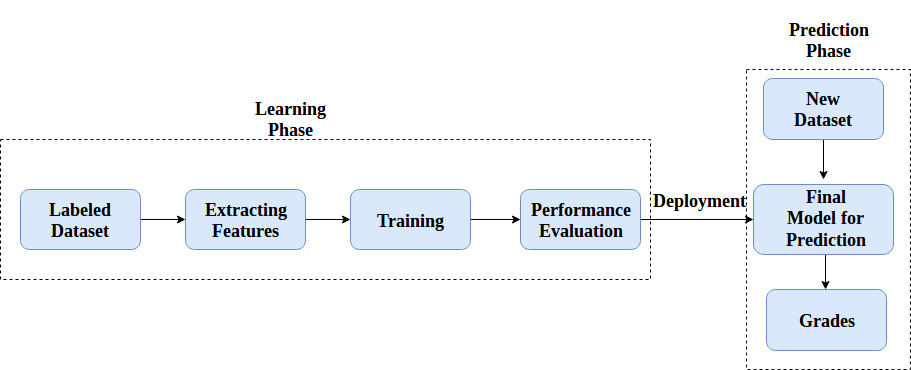
\includegraphics[scale=0.36]{images/auto_workflow}
		\caption{Workflow of automated short answer grading \cite{Burrows2015}}
		\label{auto_workflow}
	\end{figure}
\end{frame}


\subsection{Workflow of Active Learning in Automated Short Answer Grading}
\begin{frame}{Workflow of Active Learning in Automated Short Answer Grading}
	\begin{figure}[!htb]
		\centering
		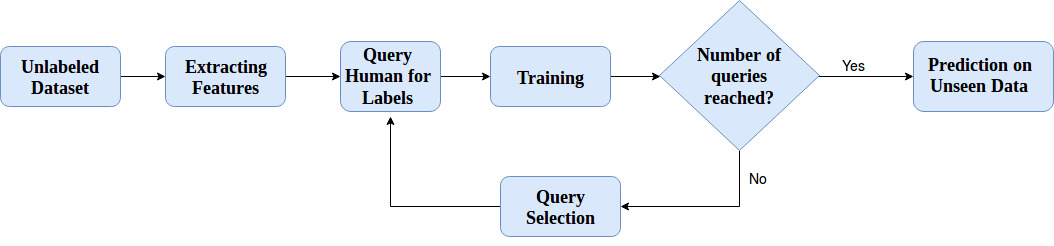
\includegraphics[scale=0.30]{images/AL_workflow}
		\caption{Workflow of active learning in automated short answer grading}
		\label{auto_workflow}
	\end{figure}
\end{frame}

\subsection{Motivation and Challenges}
\begin{frame}{Motivation and Challenges}
	
	
	\begin{columns}[T] % align columns
		\begin{column}{.48\textwidth}
			\color{blue}\rule{\linewidth}{4pt}
			Motivation
			\begin{itemize}
				\item Efficient assessment of students' response and providing feedback.
				\item Digitilization of exams.
				\item Online learning platforms.
				\item Grading is subjective in nature which could be assisted.
			\end{itemize}
		\end{column}%
		\hfill%
		\begin{column}{.48\textwidth}
			\color{blue}\rule{\linewidth}{4pt}
			
			Challenges
			\begin{itemize}
				\item Short answer grading is not a "learn once and apply forever" task.
				\item There is no single correct answer for a question. Lexical variations in students' answers need to be captured.
				\item Cost and time involved in annotating a dataset.
			\end{itemize}
		\end{column}%
	\end{columns}
	
	
	
\end{frame}

\subsection{Overview}
\begin{frame}{Overview}
	\begin{itemize}
		\item Active learning have been proved to achieve comparable results with supervised learning with less amount of labeled data in many applications \cite{dligach2011} \cite{figueroa2012}.
		\item The adaptive mechanism of active learning enables the model to learn the new input samples continuously.
		\item Different active learning settings, features, and machine learning models were evaluated on three different datasets.
		\item A web-based GUI is designed and implemented to incorporate an AI assisted short answer grading system using the best active learning setting.
	\end{itemize}
\end{frame}
%---------------------------------------------------------------

%--------------------------------------------------------------
\section{What is Active Learning?}
% First Frame
\begin{frame}{What is Active Learning?}
Active learning belongs to a special case of semi-supervised learning algorithm	where the learner is allowed to query the user to get the labels for data points which will help the learner to perform better \cite{Settles2010}.  
		\begin{figure}[!htb]
			\centering
			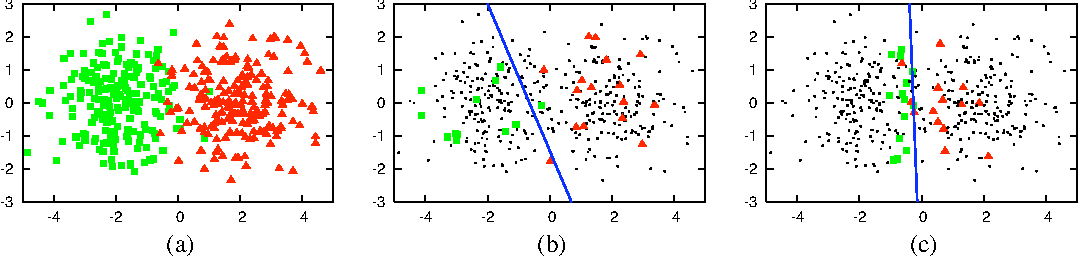
\includegraphics[scale=0.30]{images/what_ai}
			\caption{Random sampling vs Active learning. Image from \cite{Settles2010}}
			\label{auto_workflow}
		\end{figure}
	
%			\begin{figure}[!htb]
%				
%				\begin{subfigure}[b]{0.35\textwidth}
%					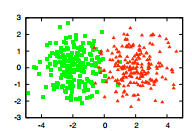
\includegraphics[width=\textwidth]{images/sample_data}
%					\caption{Data with true labels}
%					\label{sample_data}
%				\end{subfigure}
%				
%				\begin{subfigure}[b]{0.35\textwidth}
%					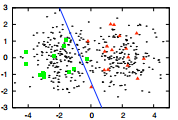
\includegraphics[width=\textwidth]{images/random_sampling}
%					\caption{Random sampling}
%					\label{random_sampling}
%				\end{subfigure}
%				~
%				\begin{subfigure}[b]{0.35\textwidth}
%					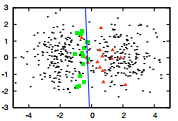
\includegraphics[width=\textwidth]{images/active_sampling}
%					\caption{Active learning}
%					\label{active_sampling}
%				\end{subfigure}
%				~
%				\caption{Random sampling vs Active learning}
%			\end{figure}
\end{frame}
%---------------------------------------------------------------





%--------------------------------------------------------------
\section{Experimental Pipeline}
% First Frame
\begin{frame}{Experimental Pipeline}
	
	\textbf{}
	
		\begin{figure}[!htb]
			\centering
			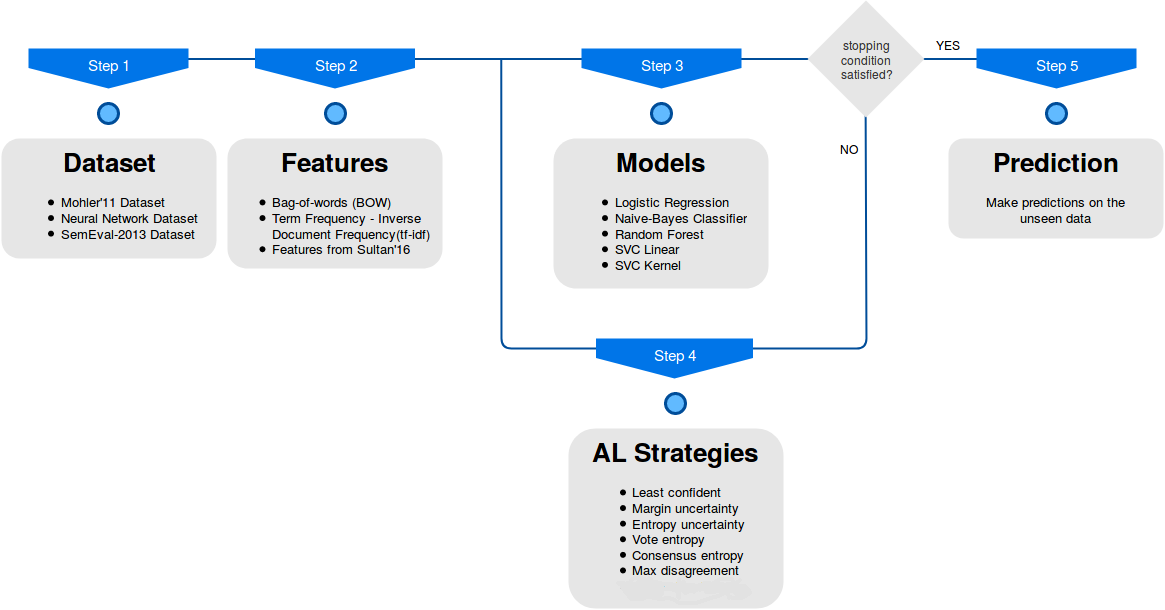
\includegraphics[scale=0.26]{images/experiment_pipeline}
			\caption{Stages of experimental pipeline}
			\label{experiment_pipeline}
		\end{figure}
\end{frame}



\subsection{Datasets}

\begin{frame}{Datasets}
\textbf{Mohler'11 Dataset \cite{Mohler2011}}
	\begin{itemize}
	\item 2273 answers from 10 assignments and 2 exams in Computer Science.
	\item The grades were normalized to 0 to 5 scale.	
	
		\begin{figure}[!htb]
			\begin{subfigure}[b]{0.35\textwidth}
				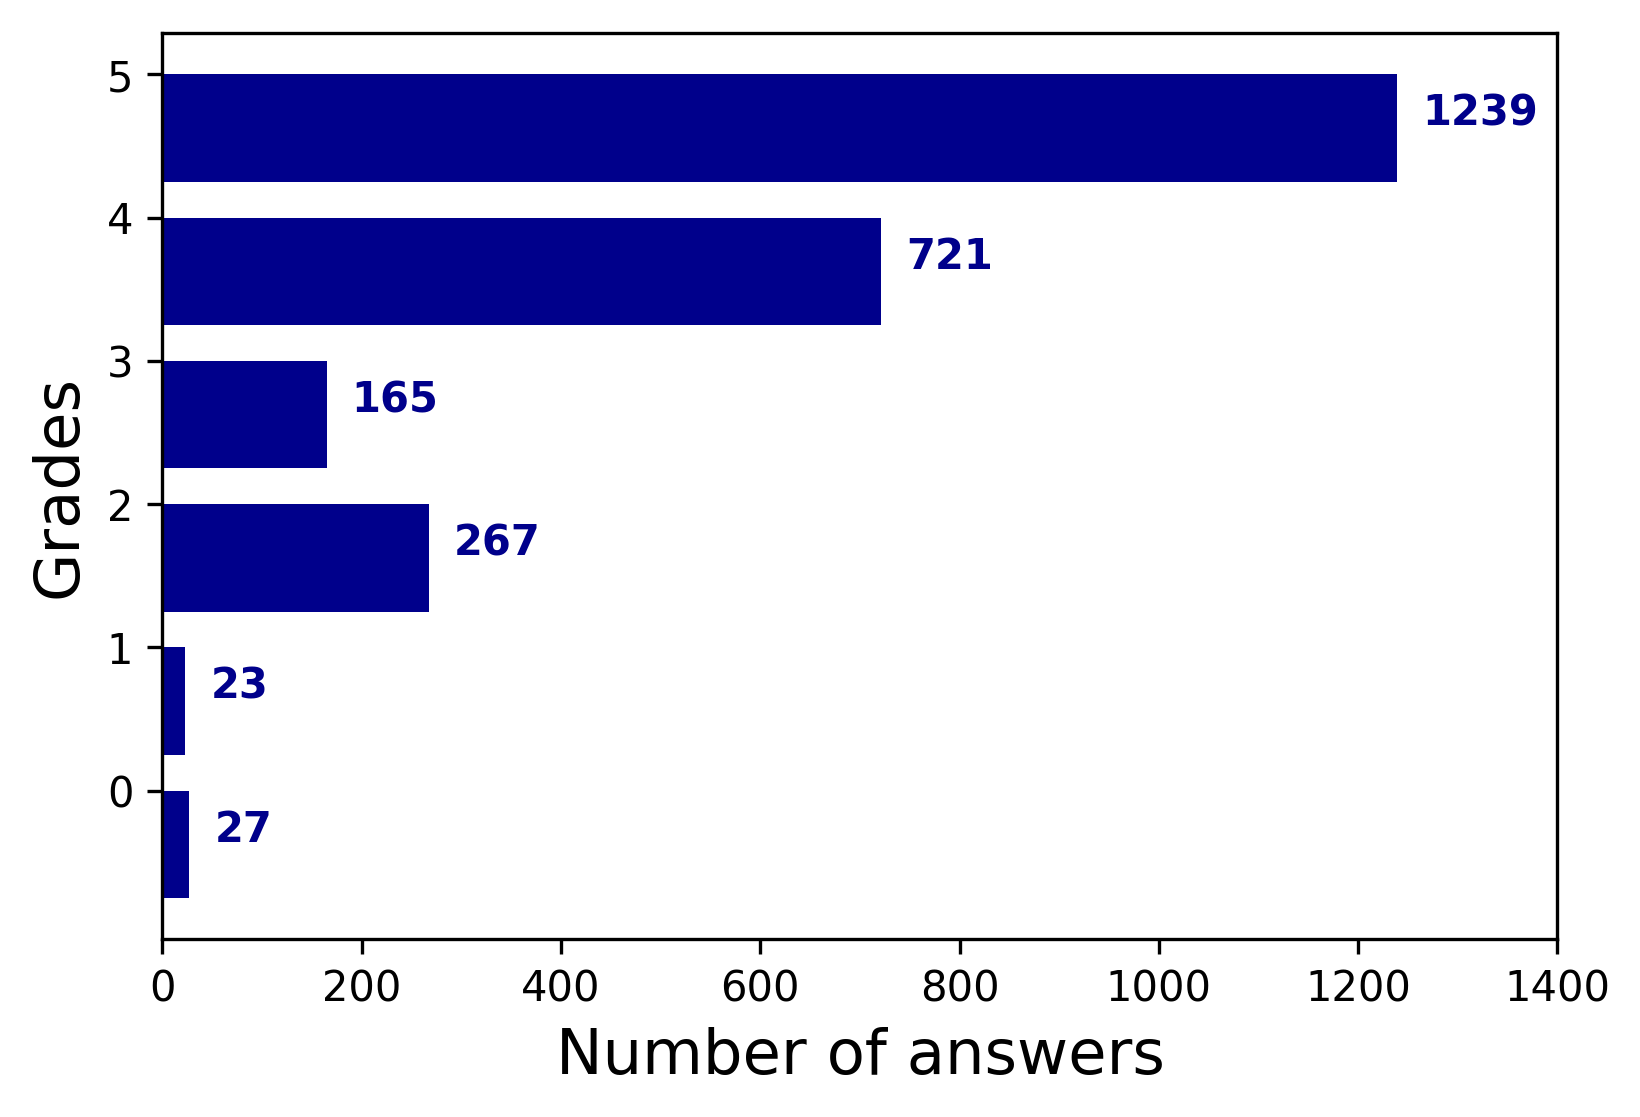
\includegraphics[width=\textwidth]{images/mohlergrades}
				\caption{Grade distribution}
				\label{mohlergrades}
			\end{subfigure}
			~
			\begin{subfigure}[b]{0.35\textwidth}
				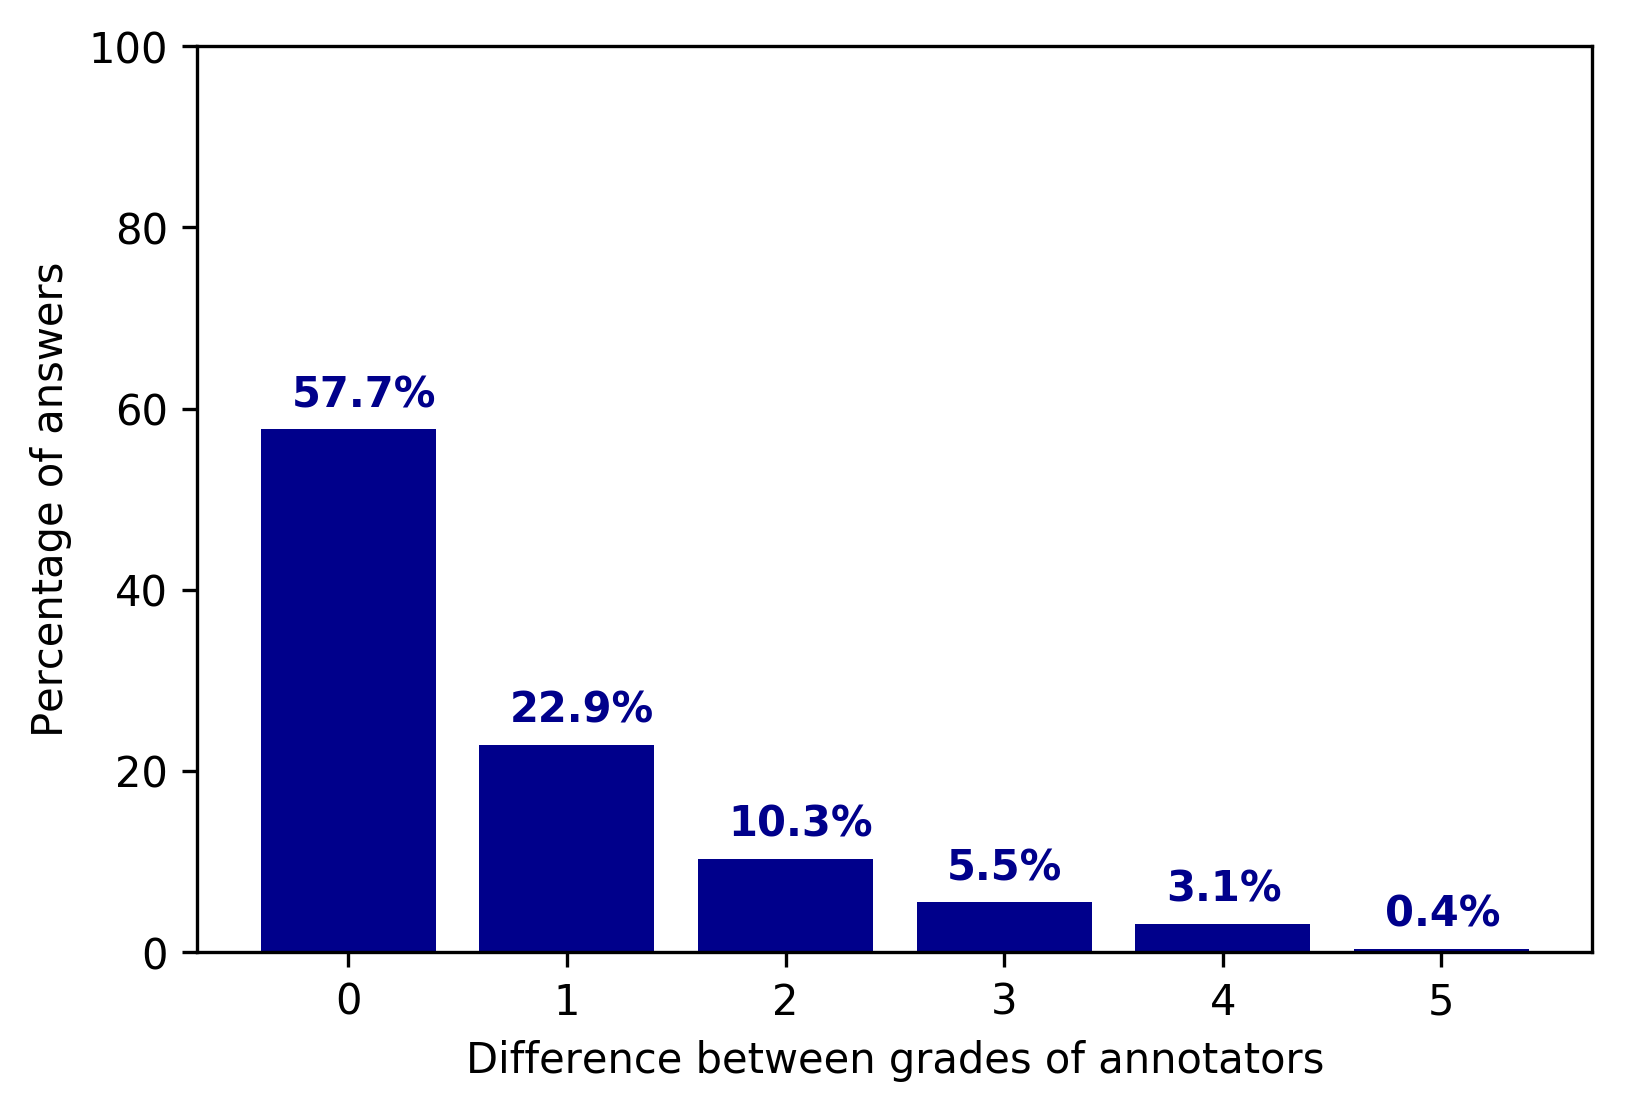
\includegraphics[width=\textwidth]{images/mohlerdisagreement}
				\caption{Inter-annotator grade analysis\cite{Mohler2011}}
				\label{mohlerdisagreement}
			\end{subfigure}
			~
			\caption{Committee-based binary classification}
		\end{figure}
	\end{itemize}
\end{frame}
\begin{frame}{Datasets}	
\textbf{Neural Network Dataset}	

\begin{itemize}
	\item Consists of 646 answers for 17 questions written by 38 students.
	\item Grades were on a scale of 0 to 2.
\end{itemize}
	\begin{figure}[!htb]
		\centering
		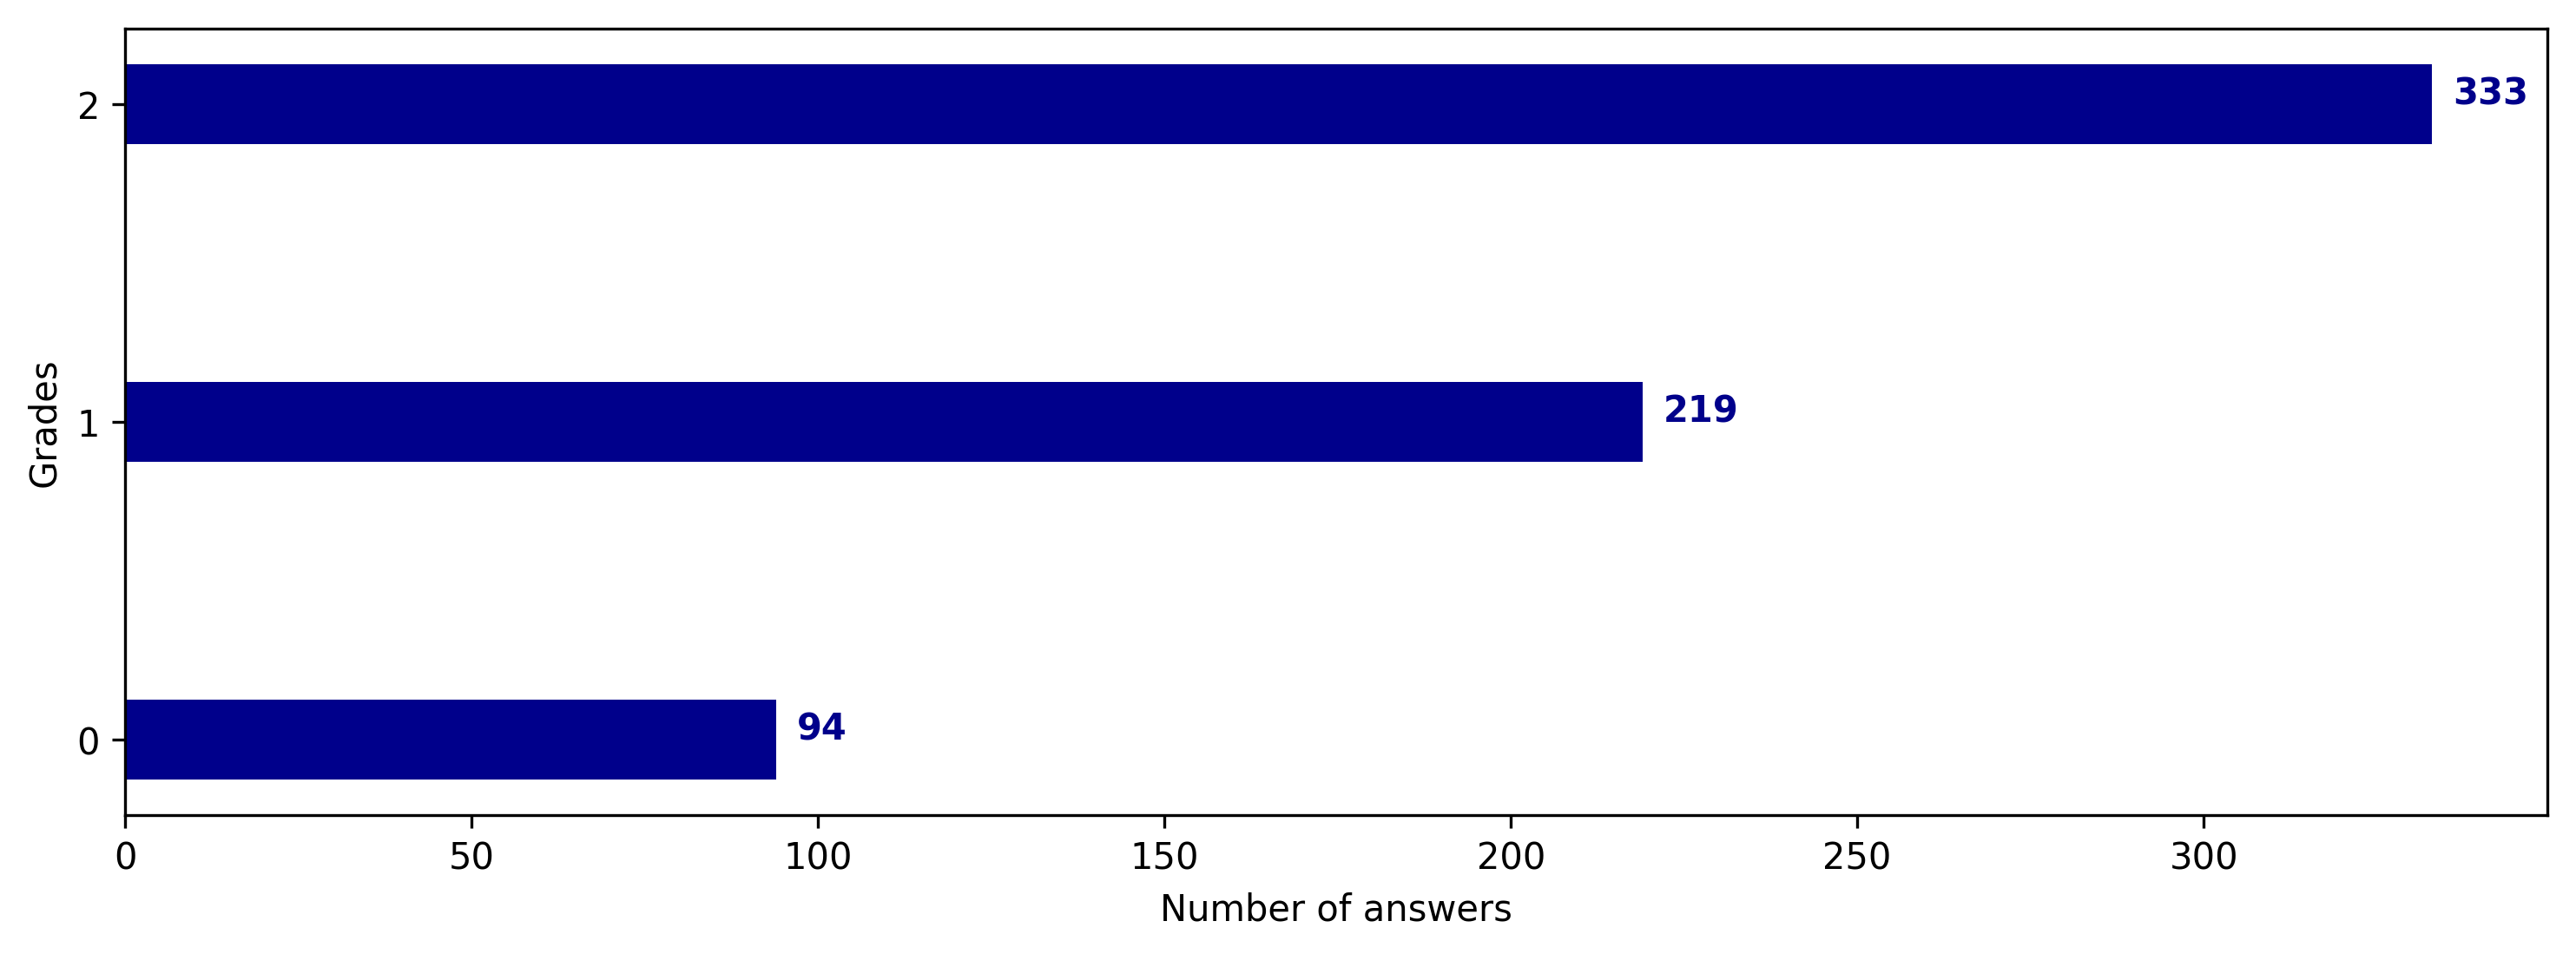
\includegraphics[scale=0.36]{images/nngrades}
		\caption{Grade distribution of NN dataset}
		\label{nngrades}
	\end{figure}
	
\end{frame}

\begin{frame}{Datasets}	
	\textbf{SemEval-2013 Task 7 Dataset \cite{dzikovska2013}}	
	\begin{itemize}
		\item Grades were on a scale of 0 to 4.
		\item Dataset was available in four distinct groups namely,
		\begin{itemize}
					\item Train dataset consist of 4969 answers. 
					\item 540 unseen answers for the same question.
					\item 4562 answers to unseen questions.
					\item 733 answers from completely different domain.
		\end{itemize}
	\end{itemize}
	
	
	
\end{frame}

\subsection{Feature Extraction}
\begin{frame}{Feature Extraction}
	\textbf{Pre-processing}
	\begin{itemize}
		\item Converting to lowercase
		\item Removing the punctuations
		\item Stop words removal 
		\item Lemmatization
	\end{itemize}
\end{frame}	

\begin{frame}{Feature Extraction}
	\textbf{Bag-of-Words(BOW)}
	\begin{itemize}
		\item ’artificial neural network massively parallel distributed processor’, ’artificial neural network largely parallel distributed processor’, and ’artificial neural network consists neurons'
		\item $\lbrack$ ’artificial’, ’consists’, ’distributed’, ’largely’, ’massively’, ’network’, ’neural’, ’neurons’, ’parallel’, ’processor’ $\rbrack$
		\item 
		    {\footnotesize  $$ \begin{bmatrix}
		    	1 & 0 & 1 & 0 & 1 & 1 & 1 & 0 & 1 & 1 \\
		    	1 & 0 & 1 & 1 & 0 & 1 & 1 & 0 & 1 & 1 \\
		    	1 & 1 & 0 & 0 & 0 & 1 & 1 & 1 & 0 & 0
		    	\end{bmatrix}  $$}   
	\end{itemize}
\end{frame}

\begin{frame}{Feature Extraction}
	\textbf{Term Frequency-Inverse Document Frequency (Tf-idf)}
	\begin{itemize}
		\item Tf-idf is a statistical tool to determine "how important a word is to a document in a collection or corpus" \cite{tf_idf_defi}.
		\item Term frequency - This captures the number of occurrence of a word in a document.
%		\item 	\begin{equation} tf(t,d) = \frac{\text{number of occurences of term in the document}}{\text{total number of all words in the document}} \end{equation} 
		\item Inverse document frequency - This calculates a low score to frequently occurring words and increasing the weights of the words that occur rarely.
%		\item 	\begin{equation} 
%		idf(t) = \frac{\text{total number of documents in the corpus}}{\text{number of documents with term t}} 
%		\end{equation}
%         \item 
	\begin{equation} tf-idf(t,d) = tf(t,d) \times idf(t) \end{equation} 
	\end{itemize}
\end{frame}

\begin{frame}{Feature Extraction}
	\textbf{Features from Sultan et al., 2016}
	\begin{figure}[!htb]
		\centering
		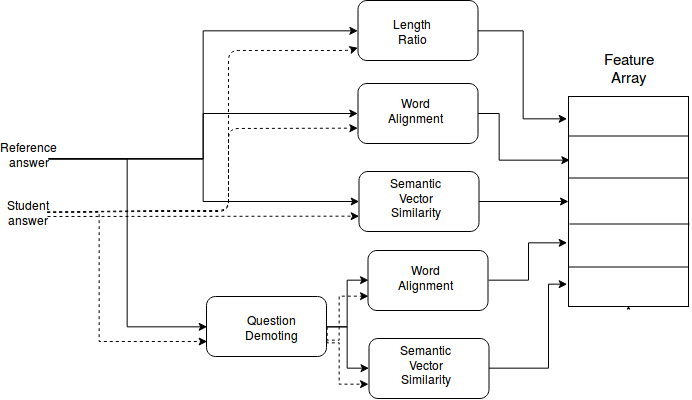
\includegraphics[scale=0.40]{images/feature_array}
		\caption{ Block diagram of construction of features from Sultan et al.,2016. Image adapted from \cite{ramesh2} \cite{Sultan2016}.}
		\label{nngrades}
	\end{figure}
\end{frame}




\subsection{Machine Learning Models}

\begin{frame}{Machine Learning Models}
	\begin{itemize}
		\item Logistic Regression
		\item Naive Bayes Classifier
		\item Random Forests
		\item Support Vector Machines
	\end{itemize}
\end{frame}




\subsection{Active Learning Query Strategies}

\begin{frame}{Active Learning Query Strategies}
	\textbf{Uncertainty Sampling}
	\begin{table}[htb!]
		\centering
		\scalebox{0.7}{
		\begin{tabular}{|c|c|c|c|}
			\hline
			\textbf{Instances} & \textbf{Class A} & \textbf{Class B} & \textbf{Class C} \\ \hline
			\textbf{I}         & 0.1              & 0.8              & 0.1              \\ \hline
			\textbf{II}        & 0.35             & 0.15             & 0.50             \\ \hline
			\textbf{III}       & 0.3              & 0.3              & 0.4              \\ \hline
		\end{tabular}}
		\caption{Prediction probabilty of three instances with respect to three classes}
		\label{least_confident}
	\end{table}
	\begin{itemize}
		\item Least confident uncertainty
		\begin{itemize}
			\item 0.2, 0.5 and 0.6
		\end{itemize}  
		\item Margin-based uncertainty
				\begin{itemize}
					\item 0.7,0.15 and 0.1
				\end{itemize} 
		\item Entropy uncertainty
		\begin{itemize}
			\item 0.64,0.99 and 1.08
		\end{itemize} 
	\end{itemize}
\end{frame}
%--------------------------------------------------------------
\begin{frame}{Active Learning Query Strategies}
	\textbf{Query-by-committee}
	\begin{itemize}
		\item Vote entropy
		\begin{table}
		
		
		\begin{subtable}{.45\textwidth}
			\centering
			\scalebox{0.7}{
			\begin{tabular}{|c|c|c|c|}
				\hline
				\textbf{Instances} & \textbf{Model 1} & \textbf{Model 2} & \textbf{Model 3} \\ \hline
				\textbf{I}         & 1                & 1                & 1                \\ \hline
				\textbf{II}        & 2                & 2                & 1                \\ \hline
				\textbf{III}       & 3                & 1                & 1                \\ \hline
				\textbf{IV}        & 1                & 2                & 3                \\ \hline
				\textbf{V}         & 2                & 2                & 1                \\ \hline
			\end{tabular}}
			\caption{Predicted labels}
			\label{vote1}
		\end{subtable}
		~
		\begin{subtable}{.45\textwidth}
			\centering
			\scalebox{0.7}{
			\begin{tabular}{|c|c|c|c|}
				\hline
				\textbf{Instances} & \textbf{Class 1} & \textbf{Class 2} & \textbf{Class 3} \\ \hline
				\textbf{I}         & 1                & 0                & 0                \\ \hline
				\textbf{II}        & 0.3333           & 0.6667           & 0                \\ \hline
				\textbf{III}       & 0.6667           & 0                & 0.3333           \\ \hline
				\textbf{IV}        & 0.3333           & 0.3333           & 0.3333           \\ \hline
				\textbf{V}         & 0.3333           & 0.6667           & 0                \\ \hline
			\end{tabular}}
			\caption{Class probability distribution}
			\label{vote2}
		\end{subtable}
		~
		\begin{subtable}{.4\textwidth}
			\centering
			\scalebox{0.7}{
			\begin{tabular}{|c|c|}
				\hline
				\textbf{Instances} & \textbf{Entropy} \\ \hline
				\textbf{I}         & 0                \\ \hline
				\textbf{II}        & 0.6365           \\ \hline
				\textbf{III}       & 0.6365           \\ \hline
				\textbf{IV}        & 1.0986           \\ \hline
				\textbf{V}         & 0.6365           \\ \hline
			\end{tabular}}
			\caption{Entropy values}
			\label{vote3}
		\end{subtable}
		\caption{Vote entropy}
	\end{table}
	\end{itemize}
\end{frame}

\begin{frame}{Active Learning Query Strategies}
	\textbf{Query-by-committee}
	\begin{itemize}
		\item Consensus entropy - Class probability averaged across each learner
		\begin{table}
		\begin{subtable}{.4\textwidth}
			\centering
			\scalebox{0.7}{
			\begin{tabular}{|c|c|c|c|}
				\hline
				\textbf{Model}   & \textbf{Class 1} & \textbf{Class 2} & \textbf{Class 3} \\ \hline
				\textbf{Model 1} & 0.6              & 0.2              & 0.2              \\ \hline
				\textbf{Model 2} & 0.5              & 0.3              & 0.2              \\ \hline
				\textbf{Model 3} & 0.55             & 0.35             & 0.1              \\ \hline
				\textbf{Model 4} & 0.1              & 0.5              & 0.4              \\ \hline
			\end{tabular}}
			\caption{Class probabilities by every model in first instance.}
			\label{con1}
		\end{subtable}
		~
				\begin{subtable}{.4\textwidth}
					\centering
					\scalebox{0.7}{
						\begin{tabular}{|c|c|c|c|}
							\hline
							\textbf{Model}   & \textbf{Class 1} & \textbf{Class 2} & \textbf{Class 3} \\ \hline
							\textbf{Model 1} & 0.3              & 0.2              & 0.5              \\ \hline
							\textbf{Model 2} & 0.3              & 0.5              & 0.2              \\ \hline
							\textbf{Model 3} & 0.35             & 0.15             & 0.5              \\ \hline
							\textbf{Model 4} & 0.2              & 0.3              & 0.5              \\ \hline
						\end{tabular}}
						\caption{Class probabilities by every model in second instance.}
						\label{con3}
					\end{subtable}
					
		\begin{subtable}{.4\textwidth}
			\centering
			\scalebox{0.7}{
			\begin{tabular}{|c|c|c|c|}
				\hline
				\textbf{Class 1} & \textbf{Class 2} & \textbf{Class 3} & \textbf{Entropy} \\ \hline
				0.44             & 0.34             & 0.22              & 1.06            \\ \hline
			\end{tabular}}
			\caption{Consensus probability for each class of the first instance.}
			\label{con2}
		\end{subtable}
		~
		\begin{subtable}{.4\textwidth}
			\centering
			\scalebox{0.7}{
			\begin{tabular}{|c|c|c|c|}
				\hline
				\textbf{Class 1} & \textbf{Class 2} & \textbf{Class 3} & \textbf{Entropy} \\ \hline
				0.29             & 0.29             & 0.42             & 1.08            \\ \hline
			\end{tabular}}
			\caption{Consensus probability for each class of the second instance.}
			\label{con4}
		\end{subtable} 
		\caption{Consensus entropy}
			\end{table}
	\end{itemize}
\end{frame}

%--------------------------------------------------------------

\section{Results}

\begin{frame}{Results on NN Dataset}
	\textbf{Sultan'16 Features with uncertainty sampling query strategy}
		\begin{figure}[!htb]
			\begin{subfigure}[b]{0.62\textwidth}
				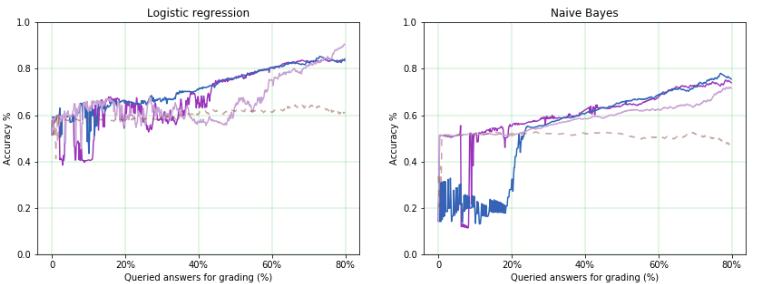
\includegraphics[width=\textwidth]{images/t1}
%				\caption{Grade distribution of mohler dataset}
				\label{mohlergrades}
			\end{subfigure}
			~
			\begin{subfigure}[b]{0.3\textwidth}
				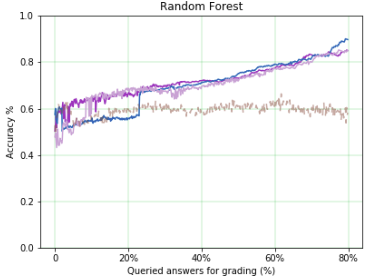
\includegraphics[width=\textwidth]{images/t2}
%				\caption{Inter-annotator grade analysis}
				\label{mohlerdisagreement}
			\end{subfigure}
			
			\begin{subfigure}[b]{0.32\textwidth}
				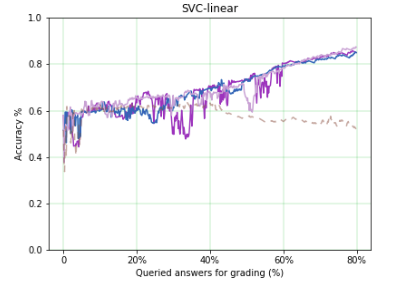
\includegraphics[width=\textwidth]{images/t3}
%				\caption{Grade distribution of mohler dataset}
				\label{mohlergrades}
			\end{subfigure}
			~
			\begin{subfigure}[b]{0.58\textwidth}
				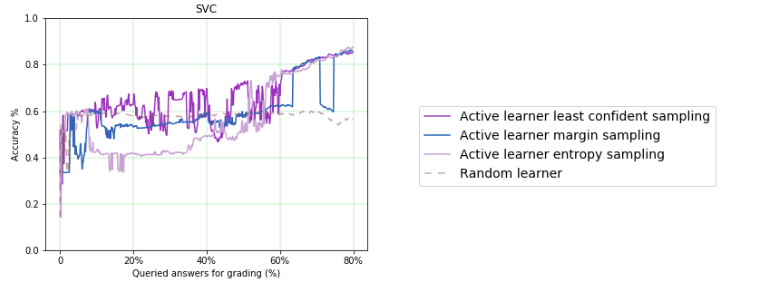
\includegraphics[width=\textwidth]{images/t4}
%				\caption{Inter-annotator grade analysis}
				\label{mohlerdisagreement}
			\end{subfigure}
			~
			\caption{Results for different models with uncertainty based query strategies}
		\end{figure}
\end{frame}

\begin{frame}
	\begin{figure}[!htb]
		\centering
		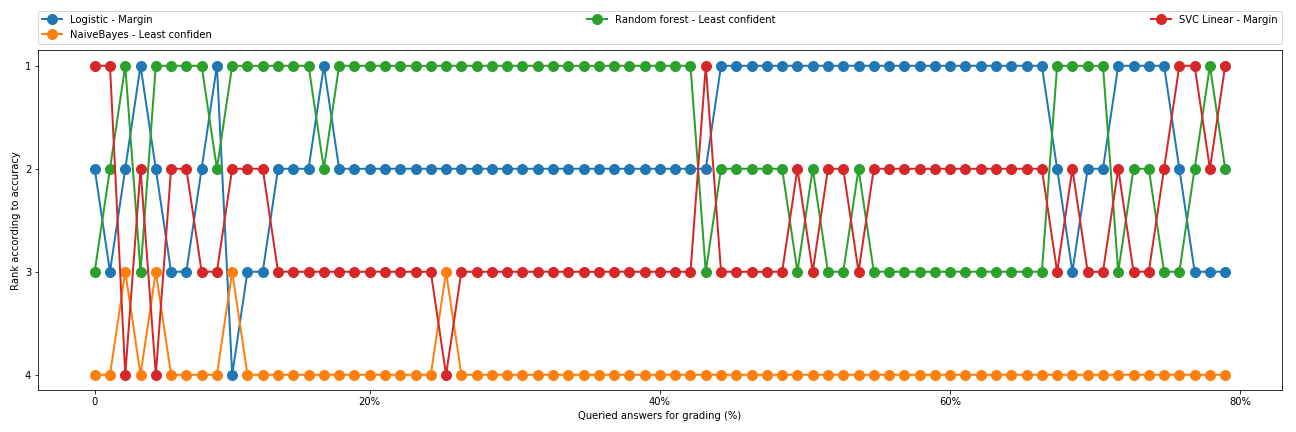
\includegraphics[scale=0.27]{images/task4_rank}
		\caption{ Bump chart of model performance in NN dataset}
		\label{nngrades}
	\end{figure}
\end{frame}
%-------------
\begin{frame}
\begin{table}[!htb]
	\centering
	\scalebox{0.75}{
		\begin{tabular}{|c|c|c|c|c|}
			\hline
			&        & Sultan                                                                    & BOW                                                              & TF-IDF                                                           \\ \hline
			\multirow{2}{*}{Mohler}   & Binary & -                                                                         & \begin{tabular}[c]{@{}c@{}}Naive Bayes -\\ Margin\end{tabular}   & \begin{tabular}[c]{@{}c@{}}Naive Bayes - \\ Margin\end{tabular}  \\ \cline{2-5} 
			& Multi  & \begin{tabular}[c]{@{}c@{}}Random Forest -\\ Least Confident\end{tabular} & \begin{tabular}[c]{@{}c@{}}Naive Bayes -\\ Margin\end{tabular}   & \begin{tabular}[c]{@{}c@{}}Naive Bayes -\\ Margin\end{tabular}   \\ \hline
			NN                        & Multi  & \begin{tabular}[c]{@{}c@{}}Random Forest -\\ Least Confident\end{tabular} & \begin{tabular}[c]{@{}c@{}}Random Forest -\\ Margin\end{tabular} & \begin{tabular}[c]{@{}c@{}}Random Forest -\\ Margin\end{tabular} \\ \hline
			\multirow{2}{*}{Sem-Eval} & Binary & \begin{tabular}[c]{@{}c@{}}Logistic Regression -\\ Margin\end{tabular}    & \begin{tabular}[c]{@{}c@{}}Random Forest -\\ Margin\end{tabular} & \begin{tabular}[c]{@{}c@{}}Random Forest -\\ Margin\end{tabular} \\ \cline{2-5} 
			& Multi  & \begin{tabular}[c]{@{}c@{}}Random Forest -\\ Least Confident\end{tabular} & \begin{tabular}[c]{@{}c@{}}Logistic Regression - \\ Margin\end{tabular}  & \begin{tabular}[c]{@{}c@{}}Logistic Regression -\\ Margin\end{tabular}   \\ \hline
		\end{tabular}}
		\caption{Best active learning settings on different datasets.}
		\label{final_comparison}
	\end{table}
\end{frame}

\begin{frame}{Supervised learning vs Active Learning}
\begin{itemize}
	\item Query strategy: Least confident uncertainty sampling
	\item Feature: Sultan'16 features
	\item Model: Random forest classifier
\end{itemize}
%	\textbf{Least confident uncertainty sampling with Sultan'16 features in random forest classifier}
			\begin{figure}[!htb]
				\begin{subfigure}[b]{0.32\textwidth}
					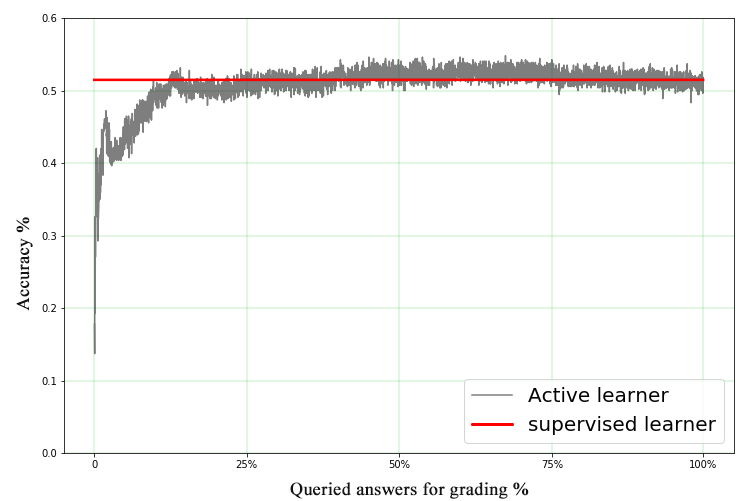
\includegraphics[width=\textwidth]{images/Unseen_Answers}
									\caption{Unseen answers}
					\label{mohlergrades}
				\end{subfigure}
			~
				\begin{subfigure}[b]{0.30\textwidth}
					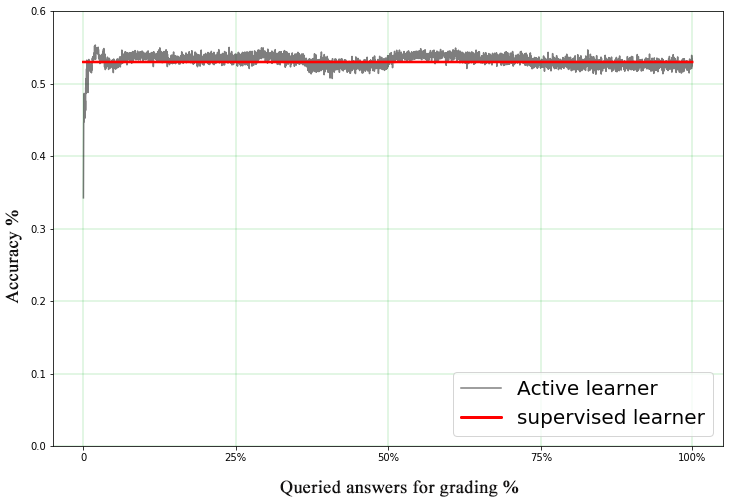
\includegraphics[width=\textwidth]{images/Unseen_Questions}
									\caption{Unseen questions}
					\label{mohlerdisagreement}
				\end{subfigure}
				~
				\begin{subfigure}[b]{0.30\textwidth}
					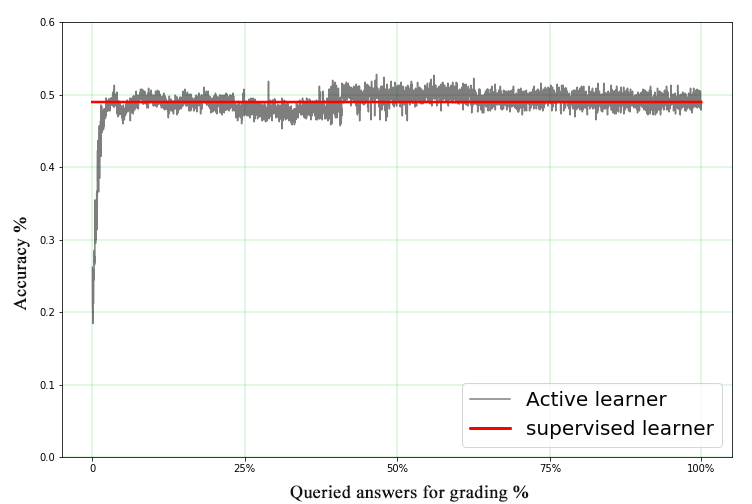
\includegraphics[width=\textwidth]{images/Unseen_Domain}
									\caption{Unseen domain}
					\label{mohlergrades}
				\end{subfigure}
				\caption{Comparison of Active learning vs Supervised learning on different datasets}
			\end{figure}
\end{frame}
\subsection{Discussions}
\begin{frame}{Discussions}
\begin{itemize}
	\item Active learning can reach the same level of performance as supervised learning with less much training data.
	\item Active learning query strategies outperformed random sampling 
	\item Least confident uncertainty query strategy with Sultan'16 features in random forest classifier performs better than other settings.
	\begin{itemize}
		\item Features require reference answer for every question. 
		\item Extracting the features is time-consuming.
	\end{itemize}
	\item Margin based uncertainty sampling worked well when bag of words or Tf-Idf features were used.
	\item Batch size of 1 and equal seeding is is found to be efficient in this task.
	
\end{itemize}	
\end{frame}
%--------------------------------------------------------------

\section{AI Assisted Grading System}


\subsection{AI Assisted Grading System}

\begin{frame}{System Architecture}
	    	\begin{figure}[!htb]
	    		\centering
	    		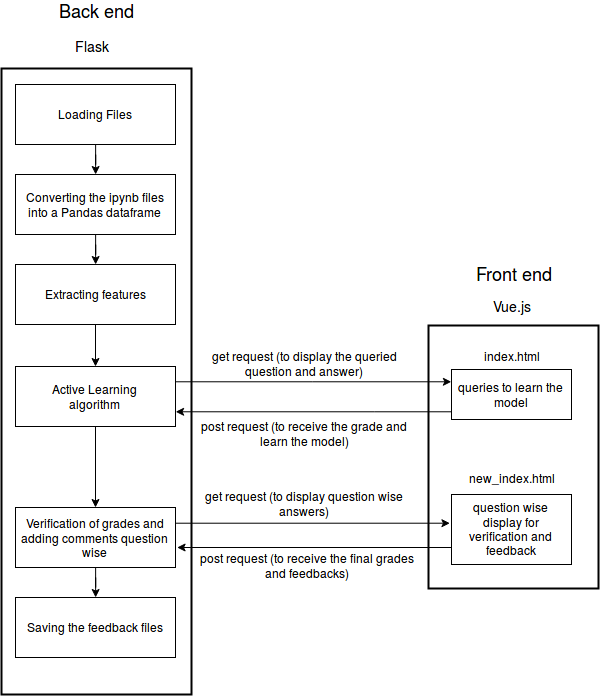
\includegraphics[scale=0.28]{images/gui_architecture}
	    		\caption{Architecture of the AI-assisted grading system (GUI).}
	    		\label{gui_architecture}
	    	\end{figure}
\end{frame}

\subsection{Number of Clicks}

\begin{frame}{Number of Clicks}
	\begin{itemize}
		\item Query Percentage: 25\%
		\item  Grading process assisted by active learning massively reduces the effort and time of the grader
	\end{itemize}
		\begin{table}[!htb]
			\centering
			\scalebox{0.75}{
				\begin{tabular}{|c|c|c|}
					\hline
					\textbf{Datasets}       & \textbf{Clicks with active learning} & \textbf{Clicks without active learning} \\ \hline
					\textbf{Neural network} & 338                                     & 680                                  \\ \hline
					\textbf{SemEval 2013}   & 3527                                    & 5104                                 \\ \hline
					\textbf{Mohler'11}      & 1386                                    & 2352                                 \\ \hline
				\end{tabular}}
				\caption{Number of clicks required to grade the answers with and without active learning.}
				\label{clicks}
			\end{table}
\end{frame}
%-------------

\section{Conclusion and future work}


\subsection{Contribution}
\begin{frame}{Contribution}
	\begin{itemize}
		\item  Detailed evaluation of different active learning settings, features and machine learning model on different datasets. 
		\item Web-based GUI which can be used for the task for grading the answers with the help of active learning.
		\item Cleaned datasets along with features are available in csv, pandas dataframe formats which could be used in future research works.
	\end{itemize}
\end{frame}


%\subsection{Lessons Learned}
%\begin{frame}{Lessons Learned}
%	\item There is no single active learning setting which would work for all the datasets.
%	
%\end{frame}

\subsection{Future Work}
\begin{frame}{Future Work}
	\begin{itemize}
		\item A study of features such as sentence embeddings and Latex embedding to improve the performance.
		\item Efficient active learning strategies to deal with skewed grade distribution in the datasets.
		\item More functionalities could be added to the GUI and can be integrated with nbgrader.
	\end{itemize}
	
\end{frame}


\begin{frame}{Acknowledgements}
	\usebeamerfont{eee}
		\begin{itemize}
			\item Active learning framework URL: \url{https://modal-python.readthedocs.io/en/latest/index.html}
			\item Word aligner URL: \url{https://github.com/rameshjesswani/Semantic-Textual-Similarity/tree/master/monolingualWordAligner}
			\item HBRS latex beamer template. URL: \url{https://git.fslab.de/mmklab/latex-templates/tree/master/presentation}
			
		\end{itemize}
\end{frame}

\begin{frame}
  \frametitle{References}
  \printbibliography[title={References}]	
\end{frame}

\begin{frame}{Demo}
\usebeamerfont{AAA}
\begin{center}	
	\begin{figure}[!htb]
		\centering
		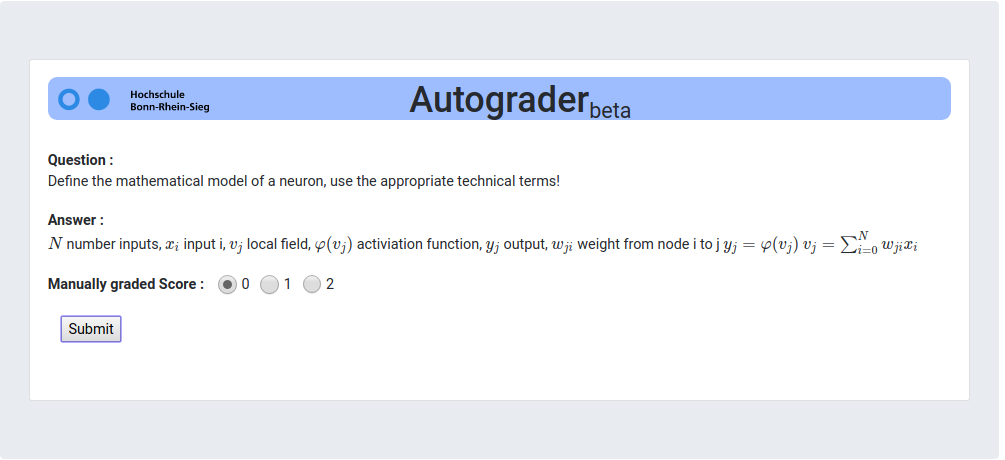
\includegraphics[scale=0.28]{images/gui_1}
%		\caption{Architecture of the AI-assisted grading system (GUI).}
		\label{gui_architecture}
	\end{figure}
\end{center}
\end{frame}

\begin{frame}{Thank you!}
	\usebeamerfont{AAA}
	\begin{center}
		Questions?
	\end{center}
\end{frame}

\end{document}
